\documentclass[12pt,a4paper,]{article}
\usepackage{pdfpages}
\usepackage{lmodern}
\usepackage{amssymb,amsmath}
\usepackage{ifxetex,ifluatex}
\usepackage{fixltx2e} % provides \textsubscript
\ifnum 0\ifxetex 1\fi\ifluatex 1\fi=0 % if pdftex
  \usepackage[T1]{fontenc}
  \usepackage[utf8]{inputenc}
\else % if luatex or xelatex
  \ifxetex
    \usepackage{mathspec}
  \else
    \usepackage{fontspec}
  \fi
  \defaultfontfeatures{Ligatures=TeX,Scale=MatchLowercase}
\fi
% use upquote if available, for straight quotes in verbatim environments
\IfFileExists{upquote.sty}{\usepackage{upquote}}{}
% use microtype if available
\IfFileExists{microtype.sty}{%
\usepackage{microtype}
\UseMicrotypeSet[protrusion]{basicmath} % disable protrusion for tt fonts
}{}
\usepackage{hyperref}
\hypersetup{unicode=true,
            pdfborder={0 0 0},
            breaklinks=true}
\urlstyle{same}  % don't use monospace font for urls
% Make links footnotes instead of hotlinks:
\renewcommand{\href}[2]{#2\footnote{See \texttt{\url{#1}}}}
\setlength{\emergencystretch}{3em}  % prevent overfull lines
\providecommand{\tightlist}{%
  \setlength{\itemsep}{0pt}\setlength{\parskip}{0pt}}
\setcounter{secnumdepth}{5}
% Redefines (sub)paragraphs to behave more like sections
\ifx\paragraph\undefined\else
\let\oldparagraph\paragraph
\renewcommand{\paragraph}[1]{\oldparagraph{#1}\mbox{}}
\fi
\ifx\subparagraph\undefined\else
\let\oldsubparagraph\subparagraph
\renewcommand{\subparagraph}[1]{\oldsubparagraph{#1}\mbox{}}
\fi

\date{}


%
% Line Spread, Page Markings & Hyperlinked Documents
%
\linespread{1.3}
% Margin:
\usepackage[top=1.5in, bottom=1.5in, right=1in, left=1in]{geometry}

% To silence too small headheight warning
\setlength{\headheight}{15pt}

% Header & Footer:
\usepackage{fancyhdr}
\pagestyle{fancy}
\fancyhf{} % Clear all header and footer fields
\fancyhead[LO,RE]{Helpdesk Ticketing System\\{\vspace{-2pt}\scriptsize Semester 2}}
\fancyhead[LE,RO]{\leftmark\\{\vspace{-4pt}\scriptsize SWE40002 Software Engineering Project}}
\fancyfoot[LE,RO]{\thepage\ifodd\value{page}\else\hfill\fi}
\usepackage{float}

\begin{document}

{
\setcounter{tocdepth}{3}
\tableofcontents
}
\newpage
\section{Doubtfire API Commits}\label{doubtfire-api}

See attached document

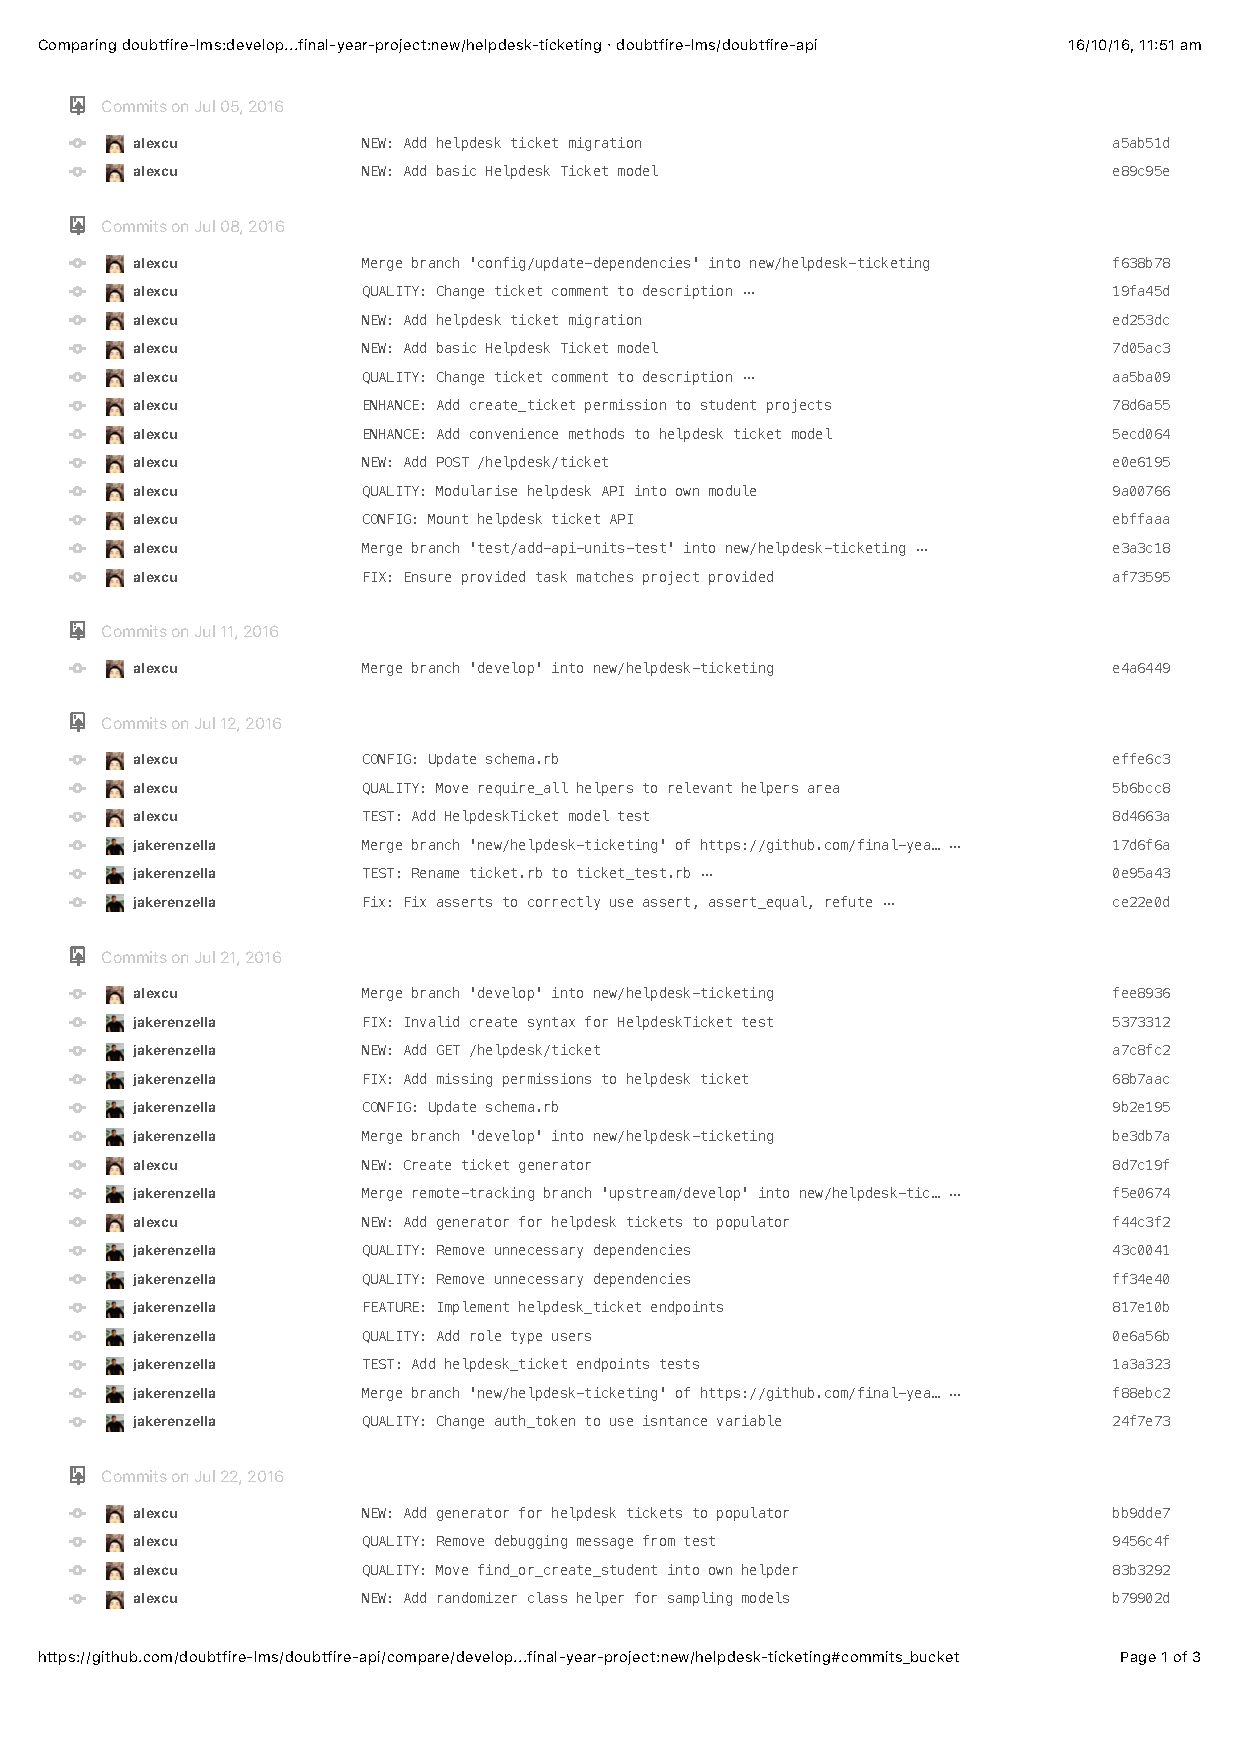
\includepdf[pages={-}]{1.pdf}

\newpage
\section{Doubtfire Web Commits}\label{doubtfire-api}

See attached document

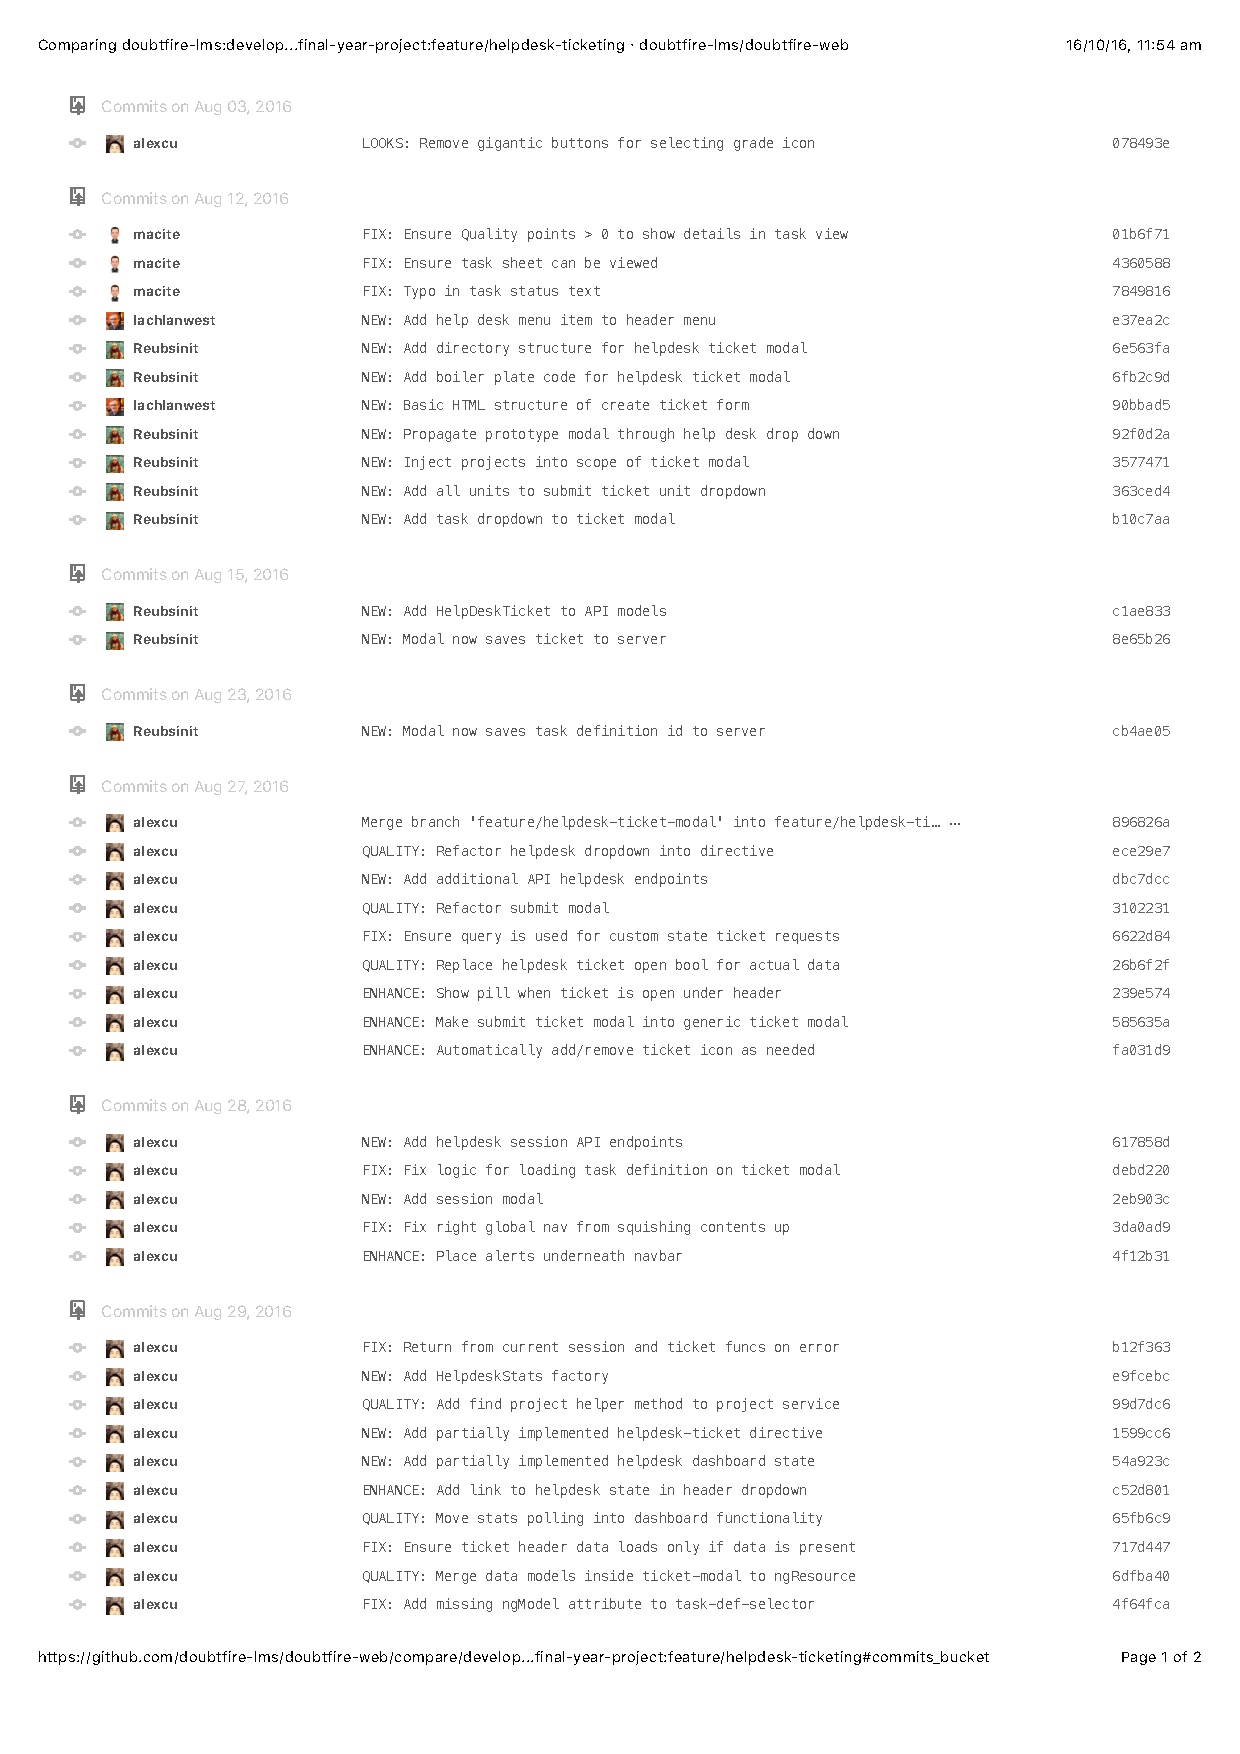
\includepdf[pages={-}]{2.pdf}

\newpage
\section{Doubtfire API Source Code Changes}\label{doubtfire-web}

See attached document

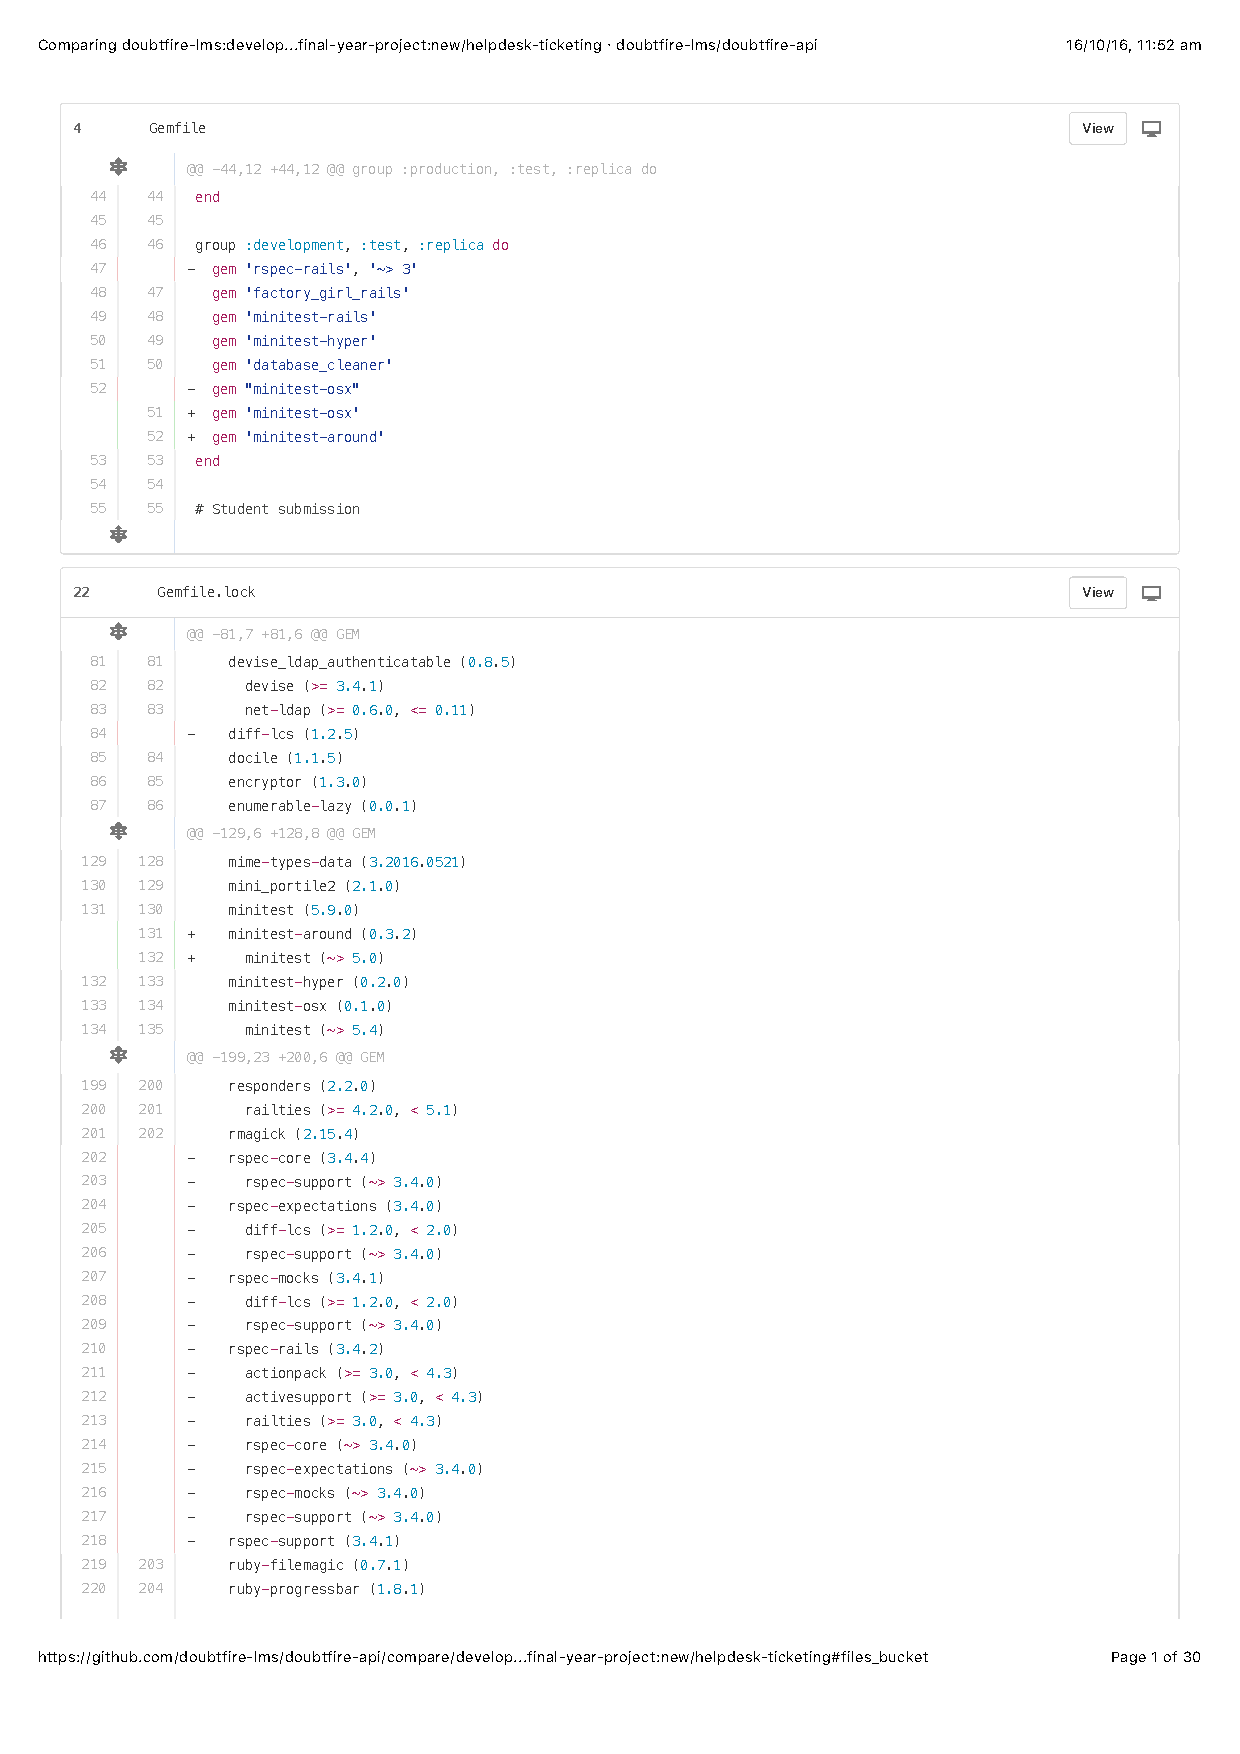
\includepdf[pages={-}]{3.pdf}

\newpage
\section{Doubtfire Web Source Code Changes}\label{doubtfire-web}

See attached document

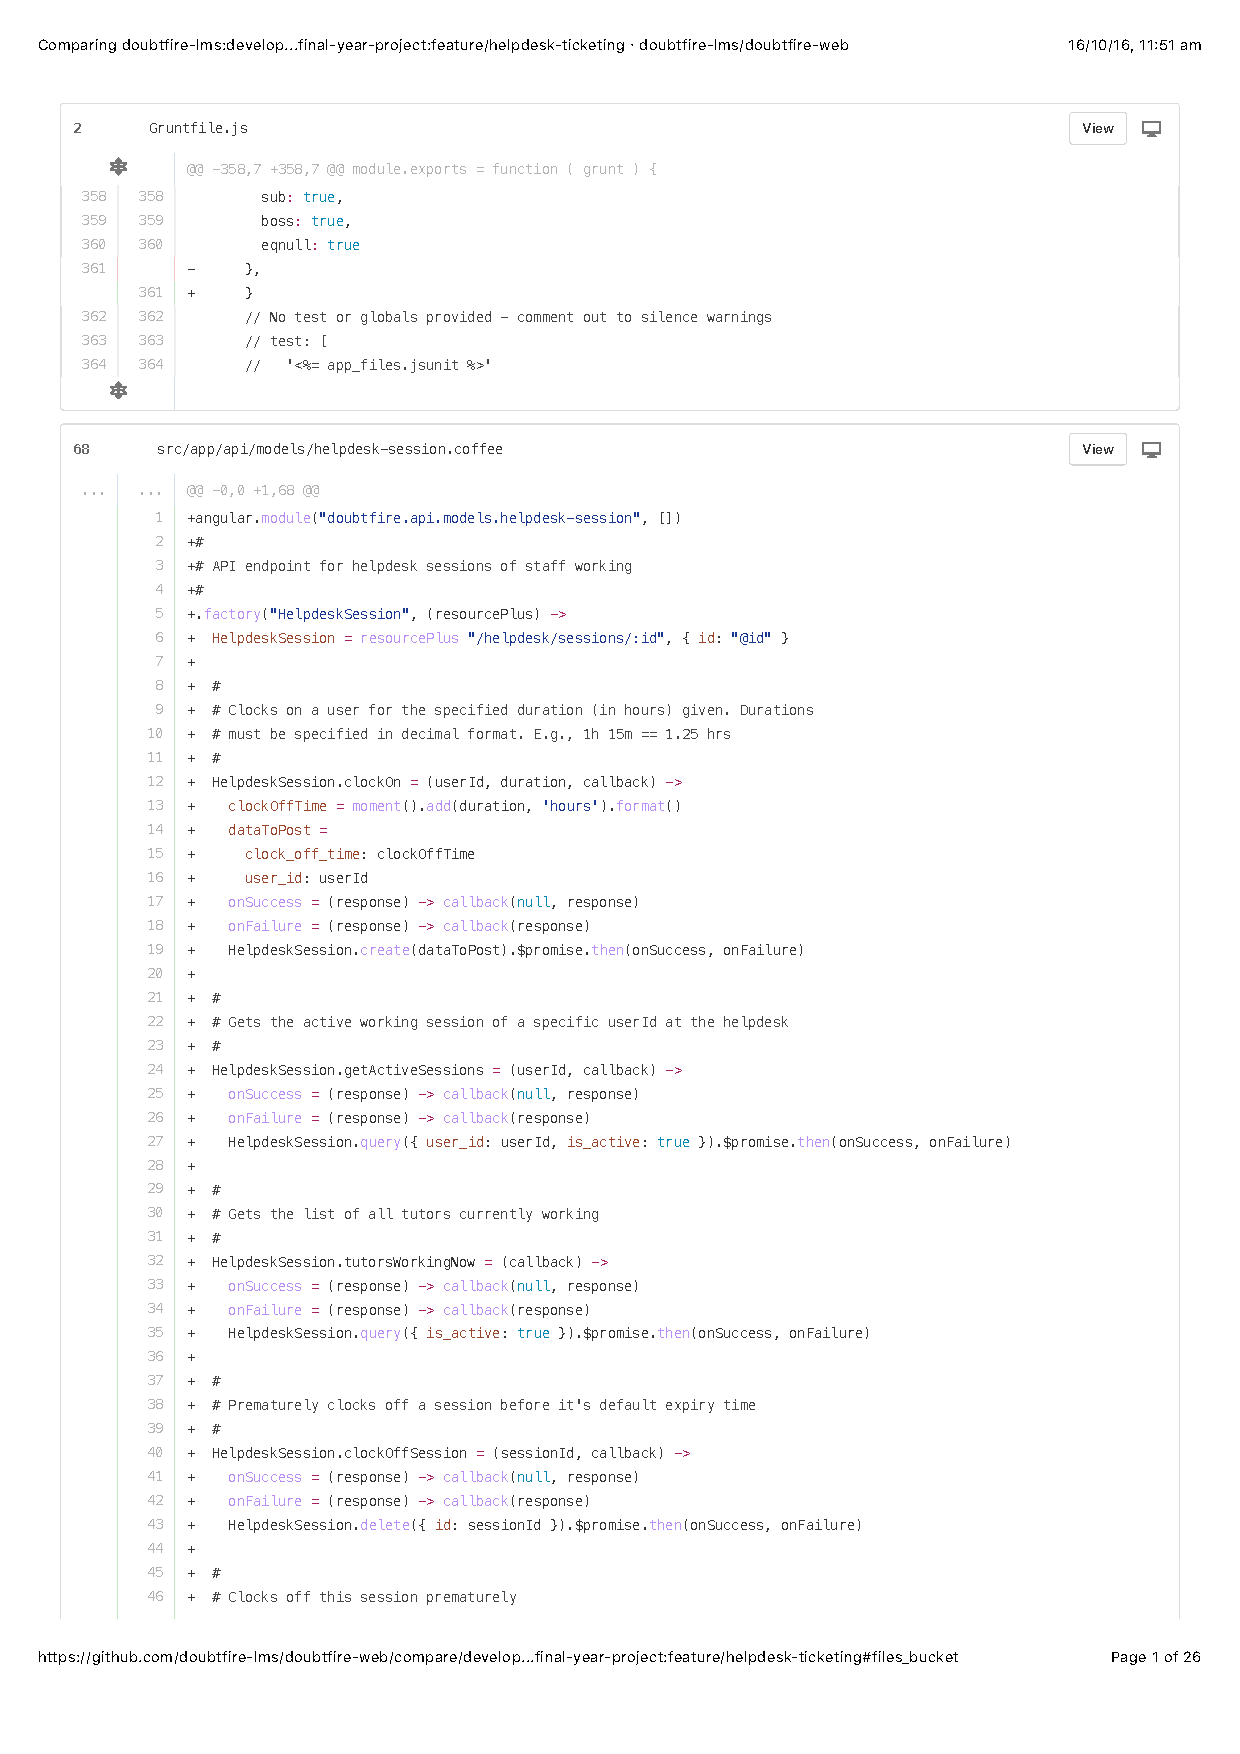
\includepdf[pages={-}]{4.pdf}

\end{document}
